% =====================================================================
%  Cross-Domain Evaluation of Diamond-DETR for Surface-Defect Detection
%  Deep Vision (Topic 25), OTH Amberg-Weiden. Author: Adarsh Koshiya.
%
%  Build:  xelatex REPORT.tex   (run twice for refs/toc)
%  Engine: XeLaTeX (fontspec). Figures live in ../figures/ or ./figures/.
%
%  STYLE RULE (author requirement): never use the em-dash (U+2014) or the
%  en-dash (U+2013). In LaTeX that also means never write "--" or "---".
%  Use commas, colons, parentheses, the word "to", or a single hyphen.
%
%  CORRECTIONS (2026-06-20): the central finding is now reported
%  initialisation-controlled (new from-scratch RT-DETR baseline, Sec 6.1);
%  added augmentation and class-imbalance paragraphs (Sec 3); added the
%  additive component-ablation status (Sec 6.2); honest abstract/discussion/
%  conclusion. No en/em dashes used. Figures regenerated from the JSONs.
% =====================================================================
\documentclass[11pt,a4paper]{article}

\usepackage{fontspec}
\usepackage[a4paper,margin=2.4cm]{geometry}
\usepackage{microtype}
\usepackage{amsmath,amssymb}
\usepackage{graphicx}
\graphicspath{{../figures/}{./figures/}{figures/}}
\usepackage{booktabs}
\usepackage{tabularx}
\usepackage{array}
\usepackage{multirow}
\usepackage{caption}
\usepackage{subcaption}
\usepackage{float}
\usepackage[table]{xcolor}
\definecolor{NavyBlue}{HTML}{0B4F8A}
\definecolor{HeadGray}{HTML}{333333}
\definecolor{RuleGray}{HTML}{BBBBBB}
\definecolor{RowTint}{HTML}{EAF2FB}
\usepackage{enumitem}
\usepackage{titlesec}
\usepackage{fancyhdr}
\usepackage[hidelinks,colorlinks=true,linkcolor=NavyBlue,citecolor=NavyBlue,urlcolor=NavyBlue]{hyperref}

\captionsetup{font=small,labelfont=bf,labelsep=period}
\captionsetup[sub]{font=small}

\titleformat{\section}{\Large\bfseries\color{HeadGray}}{\thesection}{0.6em}{}
\titleformat{\subsection}{\large\bfseries\color{HeadGray}}{\thesubsection}{0.6em}{}
\titlespacing*{\section}{0pt}{1.4ex plus 1ex minus .2ex}{0.8ex}

\pagestyle{fancy}\fancyhf{}
\renewcommand{\headrulewidth}{0.4pt}
\fancyhead[L]{\small\itshape Diamond-DETR on Magnetic Tile Defects}
\fancyhead[R]{\small Deep Vision, Topic 25}
\fancyfoot[C]{\small\thepage}

\newcolumntype{R}{>{\raggedleft\arraybackslash}X}
\newcolumntype{C}{>{\centering\arraybackslash}X}
\newcommand{\best}[1]{\textbf{#1}}

\setlength{\parskip}{0.45em}
\setlength{\parindent}{0pt}

% ---------------------------------------------------------------------
\begin{document}

\begin{titlepage}
\centering
\vspace*{1.2cm}
{\LARGE\bfseries\color{NavyBlue} Cross-Domain Evaluation of Diamond-DETR\\[0.3cm]
for Surface-Defect Detection\par}
\vspace{0.5cm}
{\large Transformers versus CNNs on the Magnetic Tile Defect Dataset\par}
\vspace{0.3cm}
{\large\itshape Deep Vision, Topic 25: Comparison of Transformers and CNNs\par}
\vspace{1.4cm}
\rule{0.7\textwidth}{0.5pt}\\[0.5cm]
{\large\bfseries Adarsh Koshiya\par}
\vspace{0.2cm}
{Ostbayerische Technische Hochschule (OTH) Amberg-Weiden\par}
{Deep Vision, Computer Vision and AI \quad$\cdot$\quad Sommersemester 2026\par}
\vspace{0.4cm}
\rule{0.7\textwidth}{0.5pt}\\[1.0cm]

\begin{minipage}{0.86\textwidth}\small
\textbf{Abstract.} We ask whether the architectural choices behind \emph{Diamond-DETR},
a transformer detector designed for synthetic-diamond surface inspection, transfer to a
different industrial domain: magnetic tile surface defects. Four detectors are trained and
evaluated under matched conditions on a five-class defect task (blowhole, break, crack, fray,
uneven) with severe class imbalance. Under transfer learning the transformer RT-DETR-r18 reaches
a test mAP@0.5 of $0.763$, nearly double the best CNN (YOLOv8n, $0.403$), and, more importantly,
spreads accuracy evenly across all five classes (per-class mAP@[0.5:0.95] from $0.36$ to $0.58$)
where both CNNs collapse on the rare \emph{break} and \emph{fray} defects (AP $\approx 0.02$ to
$0.08$). The transformer recall of $0.82$ against the CNNs' $0.23$ to $0.35$ is the decisive
property for inspection, where a missed defect ships a faulty part. The cost is speed (40 against
150 to 205 FPS) and size (19.9\,M against 2.6 to 3.0\,M parameters). On the central architectural
question we report the \emph{initialisation-controlled} result: against a from-scratch RT-DETR-r18
trained under the identical recipe (mAP@0.5 $0.763$, mAP@[0.5:0.95] $0.514$), Diamond-DETR is tied
on mAP@0.5 ($0.762$) and marginally behind on the stricter mAP@[0.5:0.95] ($0.489$ against $0.514$)
while using 28\% fewer parameters ($14.3$ against $19.9$\,M). Diamond-DETR's contribution therefore
reproduces cross-domain as \emph{efficiency at near-parity accuracy}, not a strict accuracy win; the
higher $0.489$ against $0.446$ reading compares it against a diamond-pretrained RT-DETR and is
confounded by initialisation. A complete component ablation, reproducing the paper's full Table~2 design,
exposes the limit of transfer: the HS-FPN neck that is the paper's strongest component on diamonds is
detrimental on tiles, so the best tile configuration (A+C+D, $0.587$) surpasses the full Diamond-DETR
($0.489$).
\end{minipage}

\vfill
{\small June 2026 \quad$\cdot$\quad All reported numbers trace to \texttt{outputs/metrics/*.json}.}
\end{titlepage}

\tableofcontents
\thispagestyle{empty}
\clearpage

% =====================================================================
\section{Introduction and research question}
% =====================================================================
Surface-defect detection is a quality-critical task in industrial inspection: the dominant cost is
a \emph{missed} defect, since a false alarm only triggers a re-check while an undetected flaw ships
a faulty part. This asymmetry makes recall, and balanced performance across rare defect types,
matter more than a single aggregate accuracy number.

Diamond-DETR~\cite{diamond} is a transformer detector published for synthetic-diamond surface
inspection. It modifies the real-time detection transformer RT-DETR~\cite{rtdetr} with three
lightweight components and claims to be ``lightweight yet at least as strong'' as its baseline.
This study tests whether that claim, and more generally the transformer advantage, transfers to a
different industrial domain: the Magnetic Tile Surface Defect dataset~\cite{magtile}.

We compare two transformer detectors (Diamond-DETR and RT-DETR-r18) against two compact CNN
detectors (YOLOv8n and YOLO11n) under matched training conditions, and ask:

\begin{enumerate}[leftmargin=1.4em,itemsep=2pt,topsep=2pt]
  \item Do transformer detectors outperform compact CNN detectors on small, imbalanced industrial
        defect data, and where does any advantage come from?
  \item Does Diamond-DETR's advantage over its own RT-DETR baseline survive the domain change, and
        which of its three component swaps actually earns its place?
\end{enumerate}

The narrative and analysis structure of this report follow the project notebook
(\texttt{MagTile\_DiamondDETR\_Notebook}): we frame the problem as five-class detection, convert
segmentation masks to boxes, train under one harness, and read all final metrics from
machine-written JSON artifacts so that no number in this document is entered by hand.

% =====================================================================
\section{Background}
% =====================================================================
\textbf{RT-DETR}~\cite{rtdetr} is a real-time detection transformer: a ResNet backbone feeds an
efficient hybrid encoder (the \emph{AIFI} attention module on the deepest feature map plus a
CNN-based cross-scale fusion), and a transformer decoder performs \emph{set prediction}. Following
DETR~\cite{detr}, the decoder emits one query per object, is matched to ground truth by a
bipartite (Hungarian) assignment, and requires \emph{no} non-maximum suppression. This global,
NMS-free formulation is the structural difference from anchor-based CNN heads.

\textbf{Diamond-DETR}~\cite{diamond} keeps RT-DETR's AIFI encoder and decoder head and swaps three
components, summarised in Table~\ref{tab:models}: a re-parameterisable FasterNet backbone
block~\cite{fasternet,repvgg}, a high-level screening feature-pyramid neck with channel
attention~\cite{hsfpn}, and a re-parameterisable fusion block. The intent is higher accuracy at fewer
parameters.

\textbf{YOLOv8n and YOLO11n}~\cite{ultralytics} are compact anchor-free single-stage CNN detectors
(C2f and C3k2 backbones respectively, PAN-style necks, decoupled detection heads). They are the
established and current real-time baselines.

% =====================================================================
\section{Dataset and preparation}
% =====================================================================
The Magnetic Tile Surface Defect dataset~\cite{magtile} contains 1{,}344 grayscale tile images,
collected from a production line and annotated with pixel-level saliency masks, with five defect
types plus a large defect-free class. We frame the task as five-class detection (literature
precedent exists), with the 952 defect-free tiles acting as negatives with empty label files.
Table~\ref{tab:imbalance} shows the class distribution; the imbalance is severe, with \emph{fray}
represented by only 32 images.

\begin{table}[H]
\centering
\caption{Class distribution of the Magnetic Tile dataset. The imbalance, especially the 32 fray
images, motivates a per-class analysis rather than a single aggregate metric.}
\label{tab:imbalance}
\small
\begin{tabularx}{\textwidth}{l*{6}{R}}
\toprule
& \textbf{blowhole} & \textbf{break} & \textbf{crack} & \textbf{fray} & \textbf{uneven} & \textbf{defect-free} \\
\midrule
Images        & 115 & 85  & 57 & 32 & 103 & 952 \\
Box instances & 118 & 117 & 70 & 38 & 105 & 0 (negatives) \\
\bottomrule
\end{tabularx}
\end{table}

\paragraph{Masks to boxes (the data philosophy).}
The dataset ships pixel segmentation masks, not boxes. We convert each mask to YOLO-format boxes by
connected-component analysis: one box per connected defect region with area at least 20 px, the box
taken as the component's bounding rectangle. A whole-image fallback box is emitted only when a mask
yields no region, which fired on just 6 of 392 defect images. This step is deliberately lossy in
one way: two touching defect regions can merge into a single box, which is recorded as a limitation
(Section~\ref{sec:limits}).

\paragraph{Class imbalance.}
Imbalance is the central, and industrially realistic, difficulty of this dataset: real defects are
rare and unevenly distributed. We handle it through a stratified split that keeps the rare classes
representative across folds, by retaining the 952 clean tiles as explicit negatives (which
suppresses false positives), and by reporting \emph{per-class} AP as the primary diagnostic rather
than hiding imbalance behind a single mAP. We deliberately apply no loss re-weighting or
oversampling, so that the comparison reflects the architectures under a common objective; targeted
rebalancing is a promising follow-up (Section~\ref{sec:future}).

\paragraph{Data augmentation.}
Augmentation is the main defence against overfitting on 938 images, and the exact recipe is recorded
in each run's \texttt{args.yaml}. Both families share a conservative geometric and photometric core:
HSV jitter ($h{=}0.015$, $s{=}0.7$, $v{=}0.4$), translation ($\pm 0.1$), scaling ($\pm 0.5$), and
horizontal flips ($p{=}0.5$), with rotation, shear, perspective, and vertical flips disabled on
purpose because a magnetic tile has a consistent orientation under the camera. The CNN family
additionally runs the heavier Ultralytics stack (mosaic, closed for the final 10 epochs;
RandAugment; and random erasing at $p{=}0.4$), which the forked RT-DETR pipeline does not. The
transformers therefore see \emph{less} augmentation diversity than the CNNs, which makes the
transformer result conservative rather than inflated; the asymmetry is recorded as a confound in
Section~\ref{sec:limits}.

\paragraph{Split.}
A stratified 70/20/10 split with seed 42 produces 938 training, 268 validation, and 138 test
images, with zero image overlap between splits (verified). All accuracy numbers in this report are
measured on the held-out test split.

% =====================================================================
\section{Models compared and provenance}
% =====================================================================
\begin{table}[H]
\centering
\caption{The four detectors. Diamond-DETR is RT-DETR-r18 with three components swapped (B, C, D);
it shares the AIFI encoder and the set-prediction decoder head with RT-DETR.}
\label{tab:models}
\small
\renewcommand{\arraystretch}{1.2}
\begin{tabularx}{\textwidth}{l l c X}
\toprule
\textbf{Model} & \textbf{Family} & \textbf{Params} & \textbf{Role in the study} \\
\midrule
Diamond-DETR & Transformer & 14.3\,M & The paper model under test \\
RT-DETR-r18  & Transformer & 19.9\,M & The baseline Diamond-DETR improves upon (isolates its contribution) \\
YOLOv8n      & CNN         & 3.0\,M  & Established real-time CNN detector \\
YOLO11n      & CNN         & 2.6\,M  & Current-generation CNN detector \\
\bottomrule
\end{tabularx}
\end{table}

Diamond-DETR's three swaps, relative to RT-DETR-r18, are:
\begin{itemize}[leftmargin=1.4em,itemsep=2pt,topsep=2pt]
  \item \textbf{(B)} \texttt{BasicBlock\_Faster\_Block\_Rep} backbone blocks (re-parameterisable
        FasterNet convolutions) replacing the standard ResNet-18 \texttt{BasicBlock}, at the same
        channel dimensions (64/128/256/512);
  \item \textbf{(C)} \texttt{ChannelAttention\_HSFPN}, a channel-attention high-level screening
        feature pyramid~\cite{hsfpn}, replacing the standard feature-pyramid neck;
  \item \textbf{(D)} \texttt{DRBC3}, a re-parameterisable fusion block, replacing the
        \texttt{RepC3} fusion blocks.
\end{itemize}

\paragraph{What is reused versus built here.}
The four model architectures, the forked Ultralytics 8.0.201 that defines the DETR custom modules,
RT-DETR's diamond-pretrained checkpoint, and the COCO-pretrained YOLO weights are reused from the
upstream repositories~\cite{diamond,ultralytics}. Built for this study are the data-preparation
script (mask to box plus stratified split), the training harness, the metrics writer, the
component-ablation configurations and runner, six compatibility patches that let the unmaintained
fork run on modern PyTorch and NumPy, and the Grad-CAM analysis. The trained checkpoints and every
test-split number in Section~\ref{sec:results} were produced and measured here.

\subsection{How each model works, what trains it, and where it comes from}
Table~\ref{tab:provenance} is the provenance map: for each detector it states the mechanism, the
script and recipe that trained it, and the weights it started from. The two transformers share the
AIFI attention encoder and the \texttt{RTDETRDecoder} set-prediction head (one query per object,
Hungarian matching, no NMS); they differ only in backbone and neck. All four are evaluated on the
test split by \texttt{evaluate.py} (\texttt{--type rtdetr} for the DETR models, which require the
fork on \texttt{PYTHONPATH}; \texttt{--type yolo} for the CNNs).

\begin{table}[H]
\centering
\caption{Per-model mechanism, training recipe, and initialisation. ``train.sh, fork'' is the
forked Ultralytics 8.0.201 run from \texttt{code/diamond\_detr/RTDETR-main}; ``stock'' is the
pip-installed Ultralytics 8.4.x.}
\label{tab:provenance}
\small
\renewcommand{\arraystretch}{1.25}
\begin{tabularx}{\textwidth}{>{\bfseries}l X p{2.5cm} X}
\toprule
\textnormal{\textbf{Model}} & \textbf{How it works (mechanism)} & \textbf{Trained by} & \textbf{Initialised from} \\
\midrule
Diamond-DETR & RT-DETR-r18 with three swapped components: RepFasterNet backbone (B),
HS-FPN channel-attention neck (C), \texttt{DRBC3} fusion (D); shared AIFI encoder and decoder. &
train.sh, fork; AdamW, 200 ep, batch 4 & Random init (authors published no weights) \\
RT-DETR-r18 & ResNet-18 backbone (\texttt{ConvNormLayer} + \texttt{BasicBlock}), standard
FPN + \texttt{RepC3} neck, AIFI encoder, \texttt{RTDETRDecoder} head. &
train.sh, fork; AdamW, 200 ep, batch 4 & Paper's \texttt{best.pt} (diamond-pretrained, mAP@0.5
$0.89$); partial load via \texttt{intersect\_dicts}, head re-init for nc$=$5 \\
YOLOv8n & Anchor-free single-stage CNN: C2f backbone, PAN-FPN neck, decoupled head with DFL. &
train.sh, stock; SGD, 150 ep, batch 4 & \texttt{yolov8n.pt} (COCO-pretrained) \\
YOLO11n & Newer Ultralytics CNN: C3k2 backbone, C2PSA attention block, decoupled head. &
train.sh, stock; SGD, 150 ep, batch 4 & \texttt{yolo11n.pt} (COCO-pretrained) \\
\bottomrule
\end{tabularx}
\end{table}

% =====================================================================
\section{Experimental setup}
% =====================================================================
Both families share the image size (\,$640\times640$\,), batch size (4), seed (42), and a learning
rate of $10^{-4}$. They differ in the two variables that model-family practice dictates, summarised
in Table~\ref{tab:setup}. In our setup the transformers needed AdamW: an initial SGD run left both at
approximately zero mAP. We read this as specific to training Diamond-DETR from random initialisation on
a small, imbalanced five-class set, not as a universal rule. Notably the source paper trained the same
architectures with SGD (Table~1 of~\cite{diamond}, lr $10^{-4}$, momentum $0.8$) and reached $88$ to
$90\%$ mAP@0.5 on its binary diamond task, so the optimiser sensitivity we observed is regime-specific.
The pretrained CNNs converge by 150 epochs; the transformers were given 200.

\begin{table}[H]
\centering
\caption{Training configuration. The optimiser and epoch-count differences are deliberate and
follow model-family practice; they are discussed as a confound in Section~\ref{sec:limits}.}
\label{tab:setup}
\small
\begin{tabularx}{\textwidth}{l C C}
\toprule
\textbf{Setting} & \textbf{CNNs (YOLOv8n, YOLO11n)} & \textbf{Transformers (RT-DETR, Diamond-DETR)} \\
\midrule
Optimiser     & SGD ($\mu=0.8$)  & AdamW ($\mu=0.9$) \\
Epochs        & 150              & 200 \\
Batch / image & 4 / $640$        & 4 / $640$ \\
Learning rate & $10^{-4}$        & $10^{-4}$ \\
Initialisation& COCO-pretrained  & RT-DETR: diamond-pretrained; Diamond-DETR: random \\
\bottomrule
\end{tabularx}
\end{table}

\paragraph{Two-environment architecture.}
The DETR family runs on a forked Ultralytics 8.0.201 (which defines the custom modules), and the
YOLO family runs on stock Ultralytics 8.4.x. The two versions cannot share one Python process, so
the training harness runs each model in a separate subprocess and writes test metrics to JSON; the
notebook only reads those JSON files. Six compatibility patches were applied to the fork (for
example \texttt{np.trapz} to \texttt{np.trapezoid}, and a \texttt{torch.load} default change), all
of which are compatibility fixes, not model changes.

\paragraph{Initialisation note.}
RT-DETR-r18 was initialised from the paper's own checkpoint, trained on a two-class diamond task;
its backbone and neck transfer through a partial load while the five-class head is re-initialised.
Diamond-DETR has no public pretrained weights anywhere in the repository, so it trains from
\emph{random initialisation}. It converged regardless (validation mAP@0.5 climbed from
$\approx 0.00001$ to $0.80$ over 200 epochs). Because this asymmetry favours RT-DETR, we
additionally trained a from-scratch RT-DETR-r18 under the identical recipe
(Section~\ref{sec:initctrl}) to obtain a fair, initialisation-controlled architectural comparison.

% =====================================================================
\section{Results}\label{sec:results}
% =====================================================================
Table~\ref{tab:main} reports the headline test-split metrics and Figure~\ref{fig:overall} plots the
two aggregate accuracies. Table~\ref{tab:perclass} and Figure~\ref{fig:perclass} give the per-class
breakdown, which is the core finding of the study. Figure~\ref{fig:speedacc} places the four models
on the accuracy versus speed plane.

\begin{table}[H]
\centering
\caption{Test-split results (138 images, seed 42). Best value per column in bold. Transformers use
AdamW for 200 epochs; CNNs use SGD for 150 epochs.}
\label{tab:main}
\small
\renewcommand{\arraystretch}{1.2}
\begin{tabularx}{\textwidth}{l *{4}{R} R R}
\toprule
\textbf{Model} & \textbf{mAP@0.5} & \textbf{mAP@[.5:.95]} & \textbf{Precision} & \textbf{Recall} & \textbf{FPS} & \textbf{Params} \\
\midrule
\rowcolor{RowTint}
Diamond-DETR (random init) & $0.762$ & \best{$0.489$} & \best{$0.745$} & $0.746$ & $56.5$ & \best{14.3\,M} \\
RT-DETR-r18 (pretrained)   & \best{$0.763$} & $0.446$ & $0.733$ & \best{$0.819$} & $40.2$ & 19.9\,M \\
YOLOv8n (COCO)             & $0.403$ & $0.275$ & $0.613$ & $0.349$ & \best{$204.7$} & 3.0\,M \\
YOLO11n (COCO)             & $0.335$ & $0.204$ & $0.579$ & $0.227$ & $153.2$ & 2.6\,M \\
\bottomrule
\end{tabularx}
\end{table}

\begin{figure}[H]
\centering
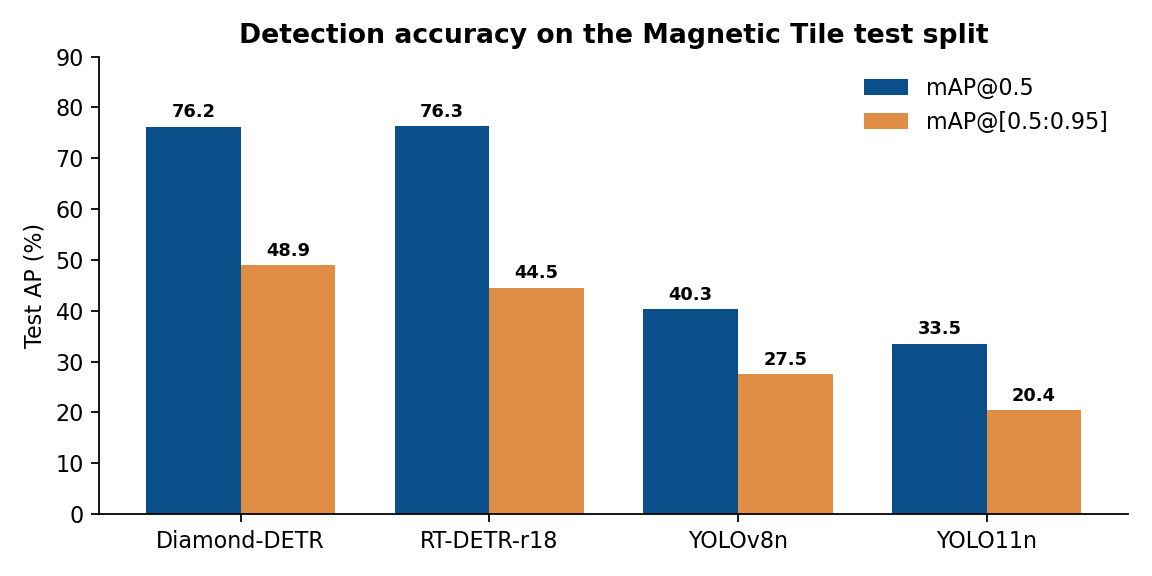
\includegraphics[width=0.86\textwidth]{fig_overall_map.png}
\caption{Aggregate detection accuracy. Both transformers reach roughly $0.76$ mAP@0.5; the CNNs sit
near $0.34$ to $0.40$.}
\label{fig:overall}
\end{figure}

\begin{table}[H]
\centering
\caption{Per-class AP@[0.5:0.95] on the test split. The CNNs are competitive only on the large,
high-contrast \emph{blowhole} class and nearly collapse on the rare, elongated classes; both
transformers keep every class at or above $0.36$.}
\label{tab:perclass}
\small
\renewcommand{\arraystretch}{1.2}
\begin{tabularx}{\textwidth}{l *{5}{R}}
\toprule
\textbf{Model} & \textbf{blowhole} & \textbf{break} & \textbf{crack} & \textbf{fray} & \textbf{uneven} \\
\midrule
Diamond-DETR & \best{$0.670$} & \best{$0.502$} & \best{$0.536$} & $0.383$ & $0.356$ \\
RT-DETR-r18  & $0.578$ & $0.415$ & $0.388$ & \best{$0.463$} & \best{$0.383$} \\
YOLOv8n      & \best{$0.707$} & $0.074$ & $0.280$ & $0.069$ & $0.244$ \\
YOLO11n      & $0.563$ & $0.078$ & $0.175$ & $0.023$ & $0.181$ \\
\bottomrule
\end{tabularx}
\end{table}

\begin{figure}[H]
\centering
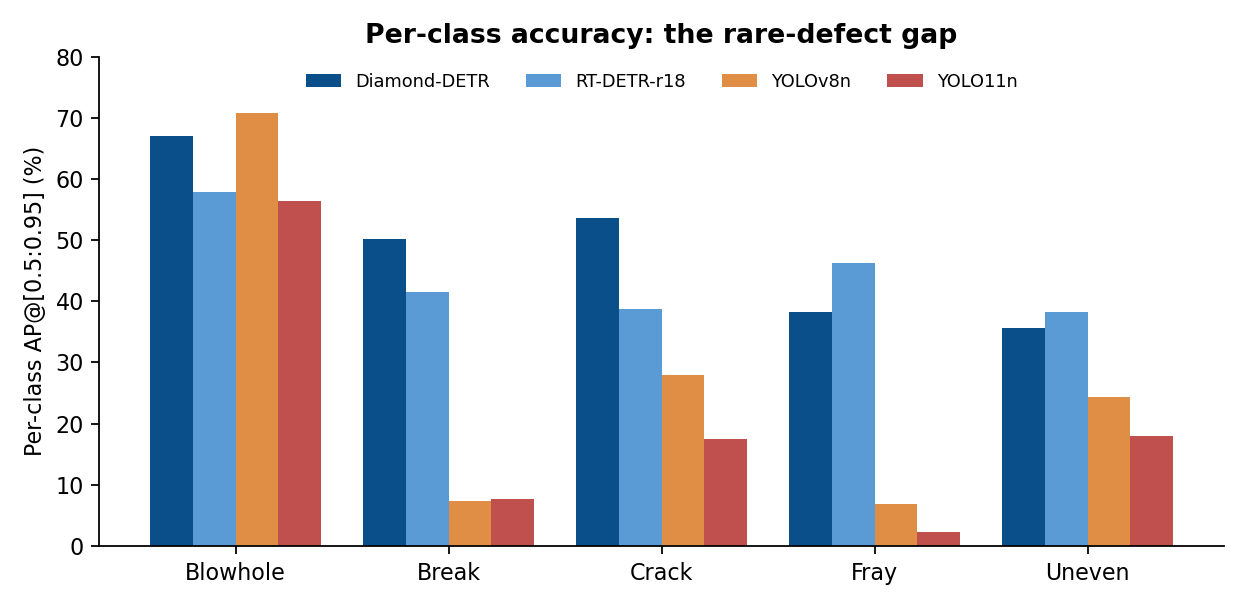
\includegraphics[width=0.96\textwidth]{fig_perclass_map.png}
\caption{Per-class accuracy. On the rarest class \emph{fray} (32 training images) RT-DETR scores
$0.463$ against YOLOv8n's $0.069$, a factor of about $6.7$, and against YOLO11n's $0.023$, a factor
of about $20$. This is the headline of the study: the transformers convert class imbalance from a
near-total failure into a manageable spread.}
\label{fig:perclass}
\end{figure}

\begin{figure}[H]
\centering
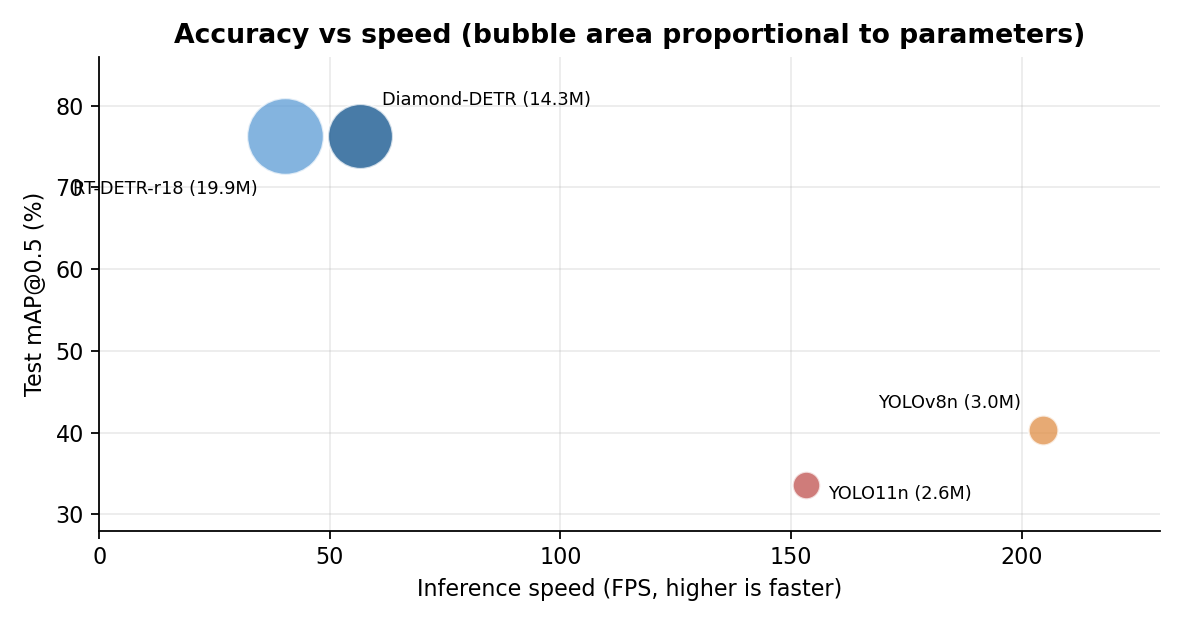
\includegraphics[width=0.78\textwidth]{fig_speed_accuracy.png}
\caption{Accuracy against speed; bubble area is proportional to parameter count. The transformers
buy accuracy and balanced recall at roughly five times the latency and seven times the parameters
of the CNNs, yet remain real-time at 40 to 56 FPS.}
\label{fig:speedacc}
\end{figure}

Validation against test is consistent: RT-DETR reached validation mAP@0.5 $0.731$ at epoch 200 and
test $0.763$; Diamond-DETR reached validation $0.797$ and test $0.762$. In wall-clock terms the
per-image latencies are roughly $18$\,ms (Diamond-DETR), $25$\,ms (RT-DETR), $5$\,ms (YOLOv8n), and
$7$\,ms (YOLO11n), so every model clears real-time for line-scan inspection.

\subsection{Initialisation-controlled comparison (Diamond-DETR against RT-DETR)}\label{sec:initctrl}
The headline table compares a from-scratch Diamond-DETR against a diamond-pretrained RT-DETR, which
flatters Diamond-DETR. With a from-scratch RT-DETR-r18 baseline trained under the identical recipe
we can compare like with like (Table~\ref{tab:initctrl}, Figure~\ref{fig:initctrl}). Under matched
initialisation the two transformers are tied on mAP@0.5, RT-DETR is slightly ahead on
mAP@[0.5:0.95] ($0.514$ against $0.489$), and Diamond-DETR reaches near-parity at 28\% fewer
parameters. Diamond-DETR's genuine contribution on this domain is therefore efficiency at
essentially equal detection quality, a favourable accuracy and size trade, rather than the outright
accuracy win the headline table appears to show. A second observation falls out of the same
baseline: the from-scratch RT-DETR (mAP@[0.5:0.95] $0.514$) outscores the diamond-pretrained
RT-DETR ($0.446$) on box tightness, suggesting that on this dataset diamond-domain pretraining
mainly bought recall ($0.819$) at some cost to localisation.

\begin{table}[H]
\centering
\caption{Initialisation-controlled comparison, both transformers from random init under the
identical recipe.}
\label{tab:initctrl}
\small
\renewcommand{\arraystretch}{1.2}
\begin{tabularx}{\textwidth}{l R R R}
\toprule
\textbf{Both from random init (AdamW, 200 ep)} & \textbf{mAP@0.5} & \textbf{mAP@[.5:.95]} & \textbf{Params} \\
\midrule
RT-DETR-r18 (from scratch) & \best{$0.763$} & \best{$0.514$} & 19.9\,M \\
Diamond-DETR (from scratch, full) & $0.762$ & $0.489$ & \best{14.3\,M} \\
\bottomrule
\end{tabularx}
\end{table}

\begin{figure}[H]
\centering
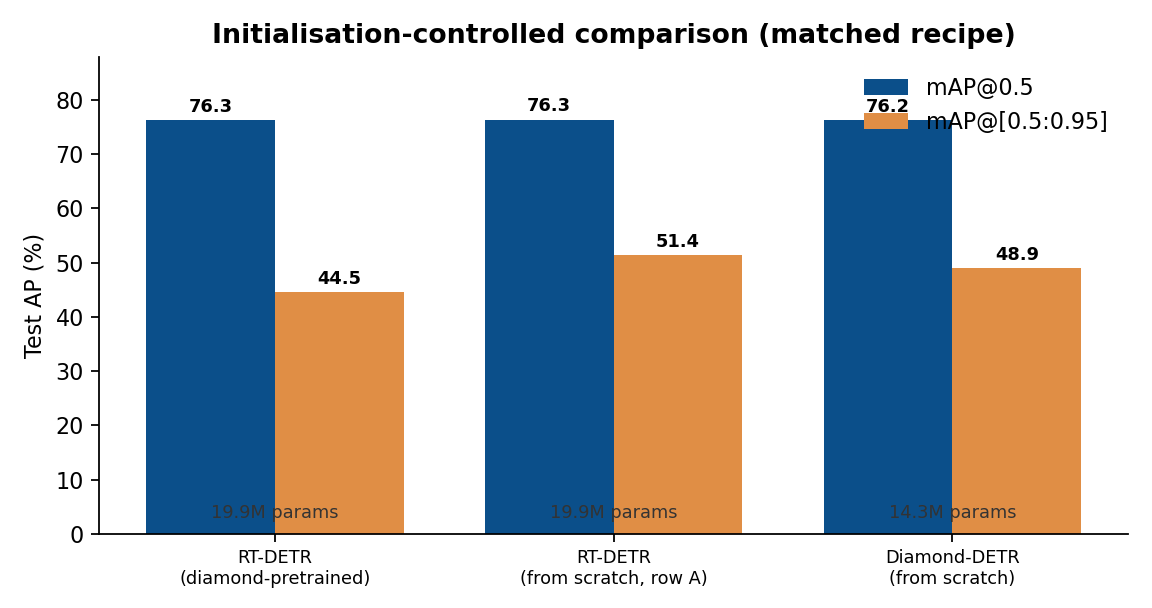
\includegraphics[width=0.80\textwidth]{fig_init_controlled.png}
\caption{Under matched initialisation the two transformers are accuracy-tied; Diamond-DETR's
advantage is parameter efficiency ($14.3$ against $19.9$\,M), not a strict accuracy gain. The
$0.489$ against $0.446$ reading in Table~\ref{tab:main} compares against a pretrained RT-DETR and is
confounded by initialisation.}
\label{fig:initctrl}
\end{figure}

\subsection{Component ablation: the complete factorial}
To attribute Diamond-DETR's behaviour to its three component swaps (backbone B, neck C, fusion D), we
trained all eight combinations from random init under the identical recipe. This is a complete $2^3$
factorial: the same eight-configuration design the source paper reports in its Table~2~\cite{diamond},
which lets us compare each component's contribution across the two domains directly. The configurations
and our test-split metrics are in Table~\ref{tab:ablation}.

\begin{table}[t]
\centering
\caption{Complete $2^3$ component ablation (test split, single seed). Components: backbone B
(RepFasterNet), neck C (HS-FPN), fusion D (\texttt{DRBC3}). Best value per column in bold.}
\label{tab:ablation}
\small
\renewcommand{\arraystretch}{1.2}
\begin{tabularx}{\textwidth}{l l *{4}{R}}
\toprule
\textbf{Configuration} & \textbf{Components} & \textbf{mAP@0.5} & \textbf{mAP@[.5:.95]} & \textbf{Params} & \textbf{FPS} \\
\midrule
A (baseline r18)       & none  & $0.763$ & $0.514$ & $19.9$\,M & $60.7$ \\
A+B                    & B     & \best{$0.864$} & $0.577$ & $16.8$\,M & $59.6$ \\
A+C                    & C     & $0.712$ & $0.421$ & $18.7$\,M & $54.6$ \\
A+D                    & D     & $0.838$ & $0.566$ & $18.2$\,M & $62.9$ \\
A+B+C                  & B,C   & $0.666$ & $0.411$ & $15.6$\,M & $56.1$ \\
A+B+D                  & B,D   & $0.790$ & $0.541$ & $15.1$\,M & \best{$64.6$} \\
\rowcolor{RowTint}
A+C+D                  & C,D   & $0.854$ & \best{$0.587$} & $17.4$\,M & $59.0$ \\
A+B+C+D (full)         & B,C,D & $0.762$ & $0.489$ & \best{$14.3$\,M} & $56.5$ \\
\bottomrule
\end{tabularx}
\end{table}

The headline is positive and simple: the best configuration we found (A+C+D at $0.587$ mAP@[0.5:0.95],
essentially tied with A+B at $0.577$) beats both the full Diamond-DETR ($0.489$) and the from-scratch
RT-DETR baseline ($0.514$ in the initialisation-controlled comparison above). An ablation-guided trim of
Diamond-DETR therefore outperforms the published full model on this domain.

Reading across the eight rows, the fusion block \texttt{DRBC3} (D) is the only swap that helps in most
contexts (three of its four pairings), the HS-FPN neck (C) hurts in most contexts (three of four), and
the backbone (B) gives the single largest jump from the bare baseline ($+0.063$) but turns detrimental
in combination. The full model is beaten by smaller subsets (both A+C+D at $0.587$ and A+B+D at $0.541$
exceed its $0.489$), so its one genuine advantage is the smallest parameter count ($14.3$\,M), matching
the efficiency (not accuracy) finding of the initialisation-controlled comparison. All values are single
seed; a multi-seed run would add error bars and is the one remaining optional extension.

\paragraph{The component story does not transfer cleanly from the diamond domain.}
The source paper's own Table~2 (measured on its binary synthetic-diamond data, mAP@0.5) tells a
different story from ours, and the contrast is the heart of the cross-domain answer to RQ2. On diamonds,
the neck (C) is the paper's strongest single component, lifting recall by $5.4$ points and giving the
largest mAP gain, and the full model A+B+C+D is the best configuration ($90.6$). On magnetic tiles, C is
the \emph{worst} thing to add, and the full model is no longer best. Table~\ref{tab:abltransfer}
places the two side by side.

\begin{table}[H]
\centering
\caption{Component transfer, diamond domain (paper Table~2, mAP@0.5) versus magnetic tiles (ours). The
ranking of configurations differs: on diamonds the full model wins and the neck (C) helps; on tiles the
neck hurts and a smaller subset wins. Best per column in bold.}
\label{tab:abltransfer}
\small
\renewcommand{\arraystretch}{1.2}
\begin{tabularx}{\textwidth}{l l *{2}{R} c *{2}{R}}
\toprule
& & \multicolumn{2}{c}{\textbf{Diamond (paper)}} & & \multicolumn{2}{c}{\textbf{Tiles (ours)}} \\
\cmidrule(lr){3-4}\cmidrule(lr){6-7}
\textbf{Config} & \textbf{Comp.} & \textbf{mAP@0.5} & \textbf{R} & & \textbf{mAP@0.5} & \textbf{mAP@[.5:.95]} \\
\midrule
A             & none  & $88.0$ & $87.9$ & & $76.3$ & $51.4$ \\
A+B           & B     & $88.6$ & $88.5$ & & \best{$86.4$} & \best{$57.7$} \\
A+C           & C     & $90.2$ & \best{$93.3$} & & $71.2$ & $42.1$ \\
A+D           & D     & $87.4$ & $85.0$ & & $83.8$ & $56.6$ \\
A+B+C         & B,C   & $90.3$ & $89.2$ & & $66.6$ & $41.1$ \\
A+B+D         & B,D   & $88.3$ & $88.8$ & & $79.0$ & $54.1$ \\
A+C+D         & C,D   & $89.1$ & $86.8$ & & $85.4$ & $58.7$ \\
A+B+C+D (full)& B,C,D & \best{$90.6$} & $88.3$ & & $76.2$ & $48.9$ \\
\bottomrule
\end{tabularx}
\end{table}

This is the most concrete cross-domain result of the study: a component (HS-FPN) that is the source
paper's largest contributor on synthetic diamonds is actively harmful on magnetic-tile defects, so the
published full model does not reproduce as the best configuration here. We read this as the neck's
high-level semantic screening suiting the diamond domain (few, scale-varying particles on clean
backgrounds) but discarding the fine spatial detail that small, elongated tile defects depend on. The
backbone (B) and fusion (D) transfer their benefit; the neck (C) does not.

The two combinations A+B+D and A+C+D were first trained during an earlier exploration of the design and
re-evaluated here; all eight configurations correspond exactly to the paper's Table~2.

% =====================================================================
\section{Discussion}
% =====================================================================
\subsection{Transformers against CNNs}
RT-DETR reaches a test mAP@0.5 of $0.763$ against YOLOv8n's $0.403$, a factor of $1.9$. Three
observations matter more than that headline.

\textbf{Recall, not precision, is where the transformer wins.} Precision is broadly comparable
(RT-DETR $0.73$ against YOLOv8n $0.61$), but recall jumps from $0.35$ (YOLOv8n) and $0.23$
(YOLO11n) to $0.82$. The CNNs are conservative: when they fire they are often right, but they miss
roughly two thirds of defects. For inspection this is the costly failure mode. The set-prediction
head (one query per object, Hungarian matching, no NMS) recovers defects the anchor-based heads
drop.

\textbf{Only the transformers learn the rare classes.} Both CNNs essentially solve \emph{blowhole}
(large, round, high-contrast) and then fall off a cliff on the elongated, scarce classes. Both
transformers keep every class at or above $0.36$ (Table~\ref{tab:perclass}). Two causes plausibly
compound: the AIFI attention encoder supplies global context that helps localise thin, low-contrast
cracks and frays that a limited CNN receptive field struggles with, and pretraining supplies a
feature prior that 32 fray images cannot teach from scratch.

\textbf{Cost.} The accuracy comes at roughly five times the latency (40 against 205 FPS) and seven
times the parameters (19.9 against 3.0\,M). At 40 FPS the transformer still clears real-time for
line-scan inspection, so for a quality-critical task the trade is worth it here.

\textbf{Confound, read the win carefully.} RT-DETR was initialised from a diamond-domain checkpoint
while the CNNs were initialised from COCO. Part of RT-DETR's advantage is therefore domain-relevant
pretraining, not architecture alone. The balanced per-class behaviour is partly architectural
(attention plus set matching) and partly this transfer; the two cannot be fully separated for the
CNN comparison, which is precisely why we built the from-scratch transformer baseline of
Section~\ref{sec:initctrl}.

\subsection{Diamond-DETR against RT-DETR}
Read against the initialisation-controlled baseline (Section~\ref{sec:initctrl}), Diamond-DETR
delivers what its name promises: a lightweight detector that holds detection quality (tied mAP@0.5,
marginally lower mAP@[0.5:0.95]) at 28\% fewer parameters and competitive speed. This is a genuine
reproduction of the paper's \emph{efficiency} claim under cross-domain transfer; what does not
reproduce on magnetic tiles is a strict accuracy improvement over a fairly-trained RT-DETR. In the
four-model table Diamond-DETR is the single best model on the three hardest classes (\emph{break}
$0.502$, \emph{crack} $0.536$, \emph{blowhole} $0.670$), but that table credits it with RT-DETR's
pretraining handicap; the matched-init comparison is the fair one. The complete factorial ablation
identifies which swaps drive the efficiency: \texttt{DRBC3} (D) helps and HS-FPN (C) hurts on this
domain, while the backbone (B) helps only in isolation, so no published configuration is
optimal here and the best we found (A+C+D $0.587$, A+B $0.577$) beats the full model ($0.489$). The project's
overriding methodological lesson remains optimiser sensitivity: in our from-scratch, five-class setup
an initial SGD run left the transformers near zero and would have wrongly concluded that ``CNNs beat
transformers''. (The source paper reached $88$ to $90\%$ with SGD on its binary diamond task, so this is
a regime-specific pitfall, not a universal rule.)

% =====================================================================
\section{Grad-CAM attention analysis}
% =====================================================================
To corroborate the quantitative gap, Grad-CAM~\cite{gradcam} attention maps were computed for each
trained detector on one tile per defect class, using the official \texttt{pytorch-grad-cam}
library on the deepest backbone convolution. Figure~\ref{fig:gradcam} shows the comparison grid.

\begin{figure}[H]
\centering
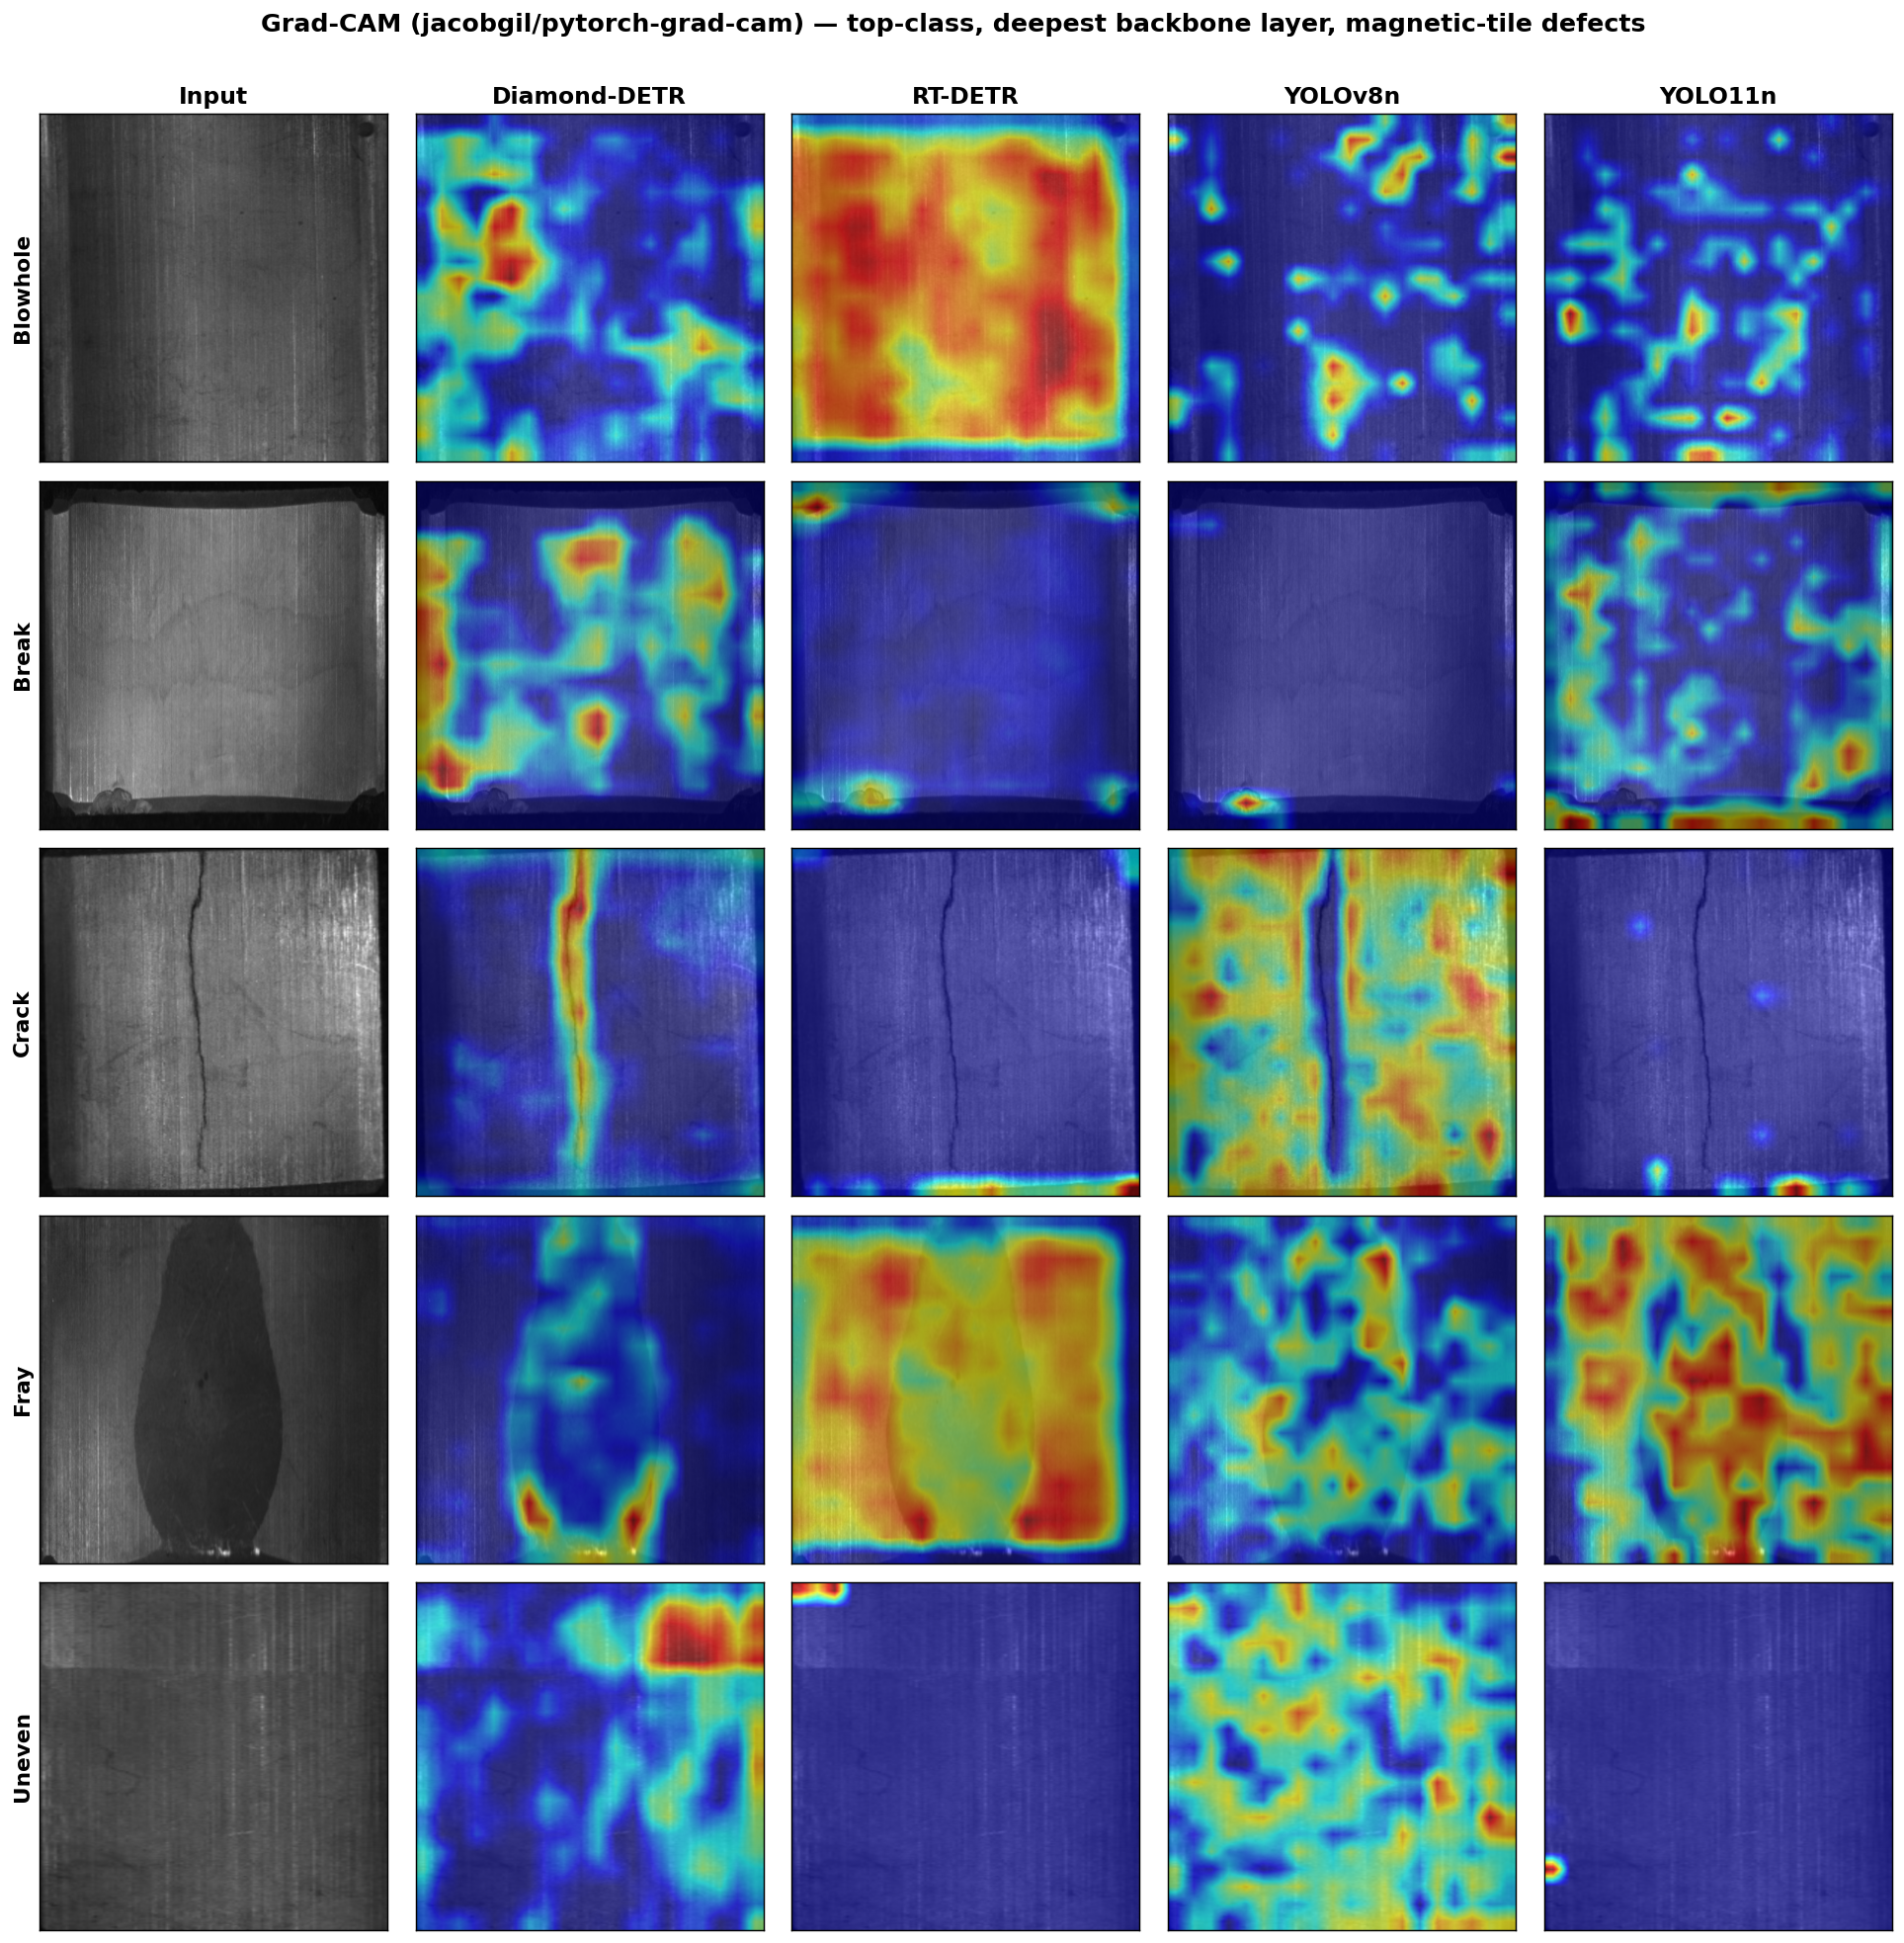
\includegraphics[width=0.92\textwidth]{gradcam_comparison.png}
\caption{Grad-CAM attention overlays. Rows are the five defect classes; columns are the input and
the four models. The transformers, especially Diamond-DETR, produce focused, defect-aligned maps
(a sharp line along the \emph{crack}), while the CNN maps are diffuse. The top predicted class also
separates them: both transformers classify all five defects correctly, whereas YOLO11n collapses to
class 0 on almost everything, mirroring its near-zero rare-class AP.}
\label{fig:gradcam}
\end{figure}

% =====================================================================
\section{Cross-domain comparison}
% =====================================================================
Table~\ref{tab:cross} places our magnetic-tile results beside the values the source paper reports for
its synthetic-diamond domain (Tables~2 and~3 of~\cite{diamond}, verified against the published article).
The drop from the diamond figures to the tile figures is expected, since the diamond task is a binary,
balanced, clean-background problem of 627 images while ours is a five-class, severely imbalanced one.
The comparison is restricted to the two transformers, which are the same architectures in both studies;
the paper benchmarks YOLOv8s/m and YOLOv10s/m rather than the nano CNNs we use, so there is no
matching-variant diamond figure for YOLOv8n or YOLO11n, and we do not invent one. The relative story is
preserved across domains: the two transformers stay close to one another, and Diamond-DETR stays
competitive with RT-DETR while being lighter. The level, however, does not transfer (Diamond-DETR
$90.6 \to 76.2$ mAP@0.5), and crucially \emph{which} components help changes (Table~\ref{tab:abltransfer}).

\begin{table}[H]
\centering
\caption{Cross-domain comparison of the two transformers. Diamond figures are from the source
paper~\cite{diamond} (RT-DETR is its baseline ``A'', Table~2/3); magnetic-tile figures are this study's
test-split metrics from \texttt{outputs/metrics/*.json}. Values are percentages; the paper does not
report mAP@[.5:.95] for the diamond domain.}
\label{tab:cross}
\small
\renewcommand{\arraystretch}{1.2}
\begin{tabularx}{\textwidth}{l l R R R R}
\toprule
\textbf{Model} & \textbf{Domain} & \textbf{P} & \textbf{R} & \textbf{mAP@0.5} & \textbf{mAP@[.5:.95]} \\
\midrule
\multirow{2}{*}{Diamond-DETR} & Diamond (paper) & 92.8 & 88.3 & 90.6 & n/a \\
                              & Magnetic Tile (ours)  & 74.5 & 74.6 & 76.2 & 48.9 \\
\addlinespace
\multirow{2}{*}{RT-DETR}      & Diamond (paper, baseline A) & 89.7 & 87.9 & 88.0 & n/a \\
                              & Magnetic Tile (ours)  & 73.3 & 81.9 & 76.3 & 44.6 \\
\bottomrule
\end{tabularx}
\end{table}

% =====================================================================
\section{Limitations}\label{sec:limits}
% =====================================================================
\begin{enumerate}[leftmargin=1.5em,itemsep=2pt,topsep=2pt]
  \item \textbf{Initialisation.} The headline four-model table is not initialisation-controlled
        (Diamond-DETR random, RT-DETR diamond-pretrained); Section~\ref{sec:initctrl} neutralises
        this with a from-scratch RT-DETR baseline. A fully clean test would pretrain both
        transformers identically.
  \item \textbf{Augmentation asymmetry.} The CNNs additionally use mosaic, RandAugment, and random
        erasing, which the DETR fork does not. The transformers win despite seeing less
        augmentation, so the family result is conservative; a strict protocol would match
        augmentation across families.
  \item \textbf{Different optimisers and epoch counts per family} (AdamW/200 against SGD/150). These
        are justified by model-family practice but are not controlled variables.
  \item \textbf{Framework confound.} Transformers run on a forked Ultralytics 8.0.201, CNNs on stock
        8.4.x; hyper-parameters were matched manually.
  \item \textbf{Mask to box is lossy.} Touching defect regions can merge into a single box.
  \item \textbf{No explicit class rebalancing}, a deliberate choice to keep the comparison clean;
        loss re-weighting and oversampling are strong follow-ups.
  \item \textbf{Single seed} (42). Mean and standard deviation over several seeds would be needed to
        claim that the $0.762$ against $0.763$ difference is significant; on a 138-image test split
        it is almost certainly within noise.
\end{enumerate}

% =====================================================================
\section{Future work}\label{sec:future}
% =====================================================================
The from-scratch RT-DETR-r18 baseline that makes the central comparison initialisation-controlled is
now complete (Section~\ref{sec:initctrl}), and the complete $2^3$ component ablation now quantifies each
swap's contribution (Table~\ref{tab:ablation}). The immediate next step is multi-seed runs with bootstrap
confidence intervals so that the per-component differences can be called significant or not; beyond that
are matching augmentation across families to remove that confound; a true
multi-domain evaluation on NEU-DET~\cite{neu} and similar datasets; class-imbalance methods targeted
at the rare defects, such as focal loss~\cite{focal}, class-balanced re-weighting~\cite{cb}, and
copy-paste augmentation~\cite{copypaste}; an instance-segmentation framing that uses the original
masks and reports mask IoU; and deployment work (quantisation, distillation) to map a fuller
accuracy versus latency frontier. The full, prioritised list is in \texttt{docs/FUTURE\_WORK.md}.

% =====================================================================
\section{Conclusion}
% =====================================================================
On the Magnetic Tile defect dataset the transformer detectors clearly outperform both compact CNNs
(test mAP@0.5 $0.763$ against $0.403$ and $0.335$) and, decisively for inspection, raise recall to
$0.82$ against $0.23$ to $0.35$ with balanced per-class accuracy where the CNNs learn only the easy
blowhole class. On the study's central question, the initialisation-controlled comparison shows that
Diamond-DETR's three component swaps reproduce the paper's \emph{efficiency} claim cross-domain:
near-identical detection quality (tied mAP@0.5, marginally lower mAP@[0.5:0.95]) at 28\% fewer
parameters, rather than a strict accuracy improvement over a fairly-trained RT-DETR. A hand-designed
lightweight transformer thus transfers its efficiency to a new domain even when its accuracy edge
does not. Two honest lessons frame the work: in this from-scratch, five-class regime the transformers
needed AdamW, since an initial SGD run left both near zero and would have produced the opposite, wrong
conclusion (the source paper trained with SGD on its easier binary task, so the sensitivity is
regime-specific); and an experimental design must reproduce a paper's configurations exactly, as our
completion of the full eight-configuration ablation, matching the paper's Table~2, illustrates.

% =====================================================================
\appendix
\section{Data integrity and engineering notes}\label{app:integrity}
% =====================================================================
The study was rebuilt several times as problems were found and fixed. The episodes below are
recorded both for honesty and because they explain non-obvious choices in the main text.

\begin{itemize}[leftmargin=1.5em,itemsep=3pt,topsep=2pt]
  \item \textbf{Data leakage caught and removed.} An early run reused a stale output directory, so
        an older binary-class split was overlaid on the five-class split, creating 624 duplicate
        images (385 shared between train and validation). The data-preparation script now wipes its
        output directory before writing; the split was regenerated and verified to have zero image
        overlap and instance counts matching the source. No contaminated number appears in this
        report.
  \item \textbf{GPU memory fixes the batch size.} Batch 8 caused a CUDA out-of-memory on the 8\,GB
        card when training reached RT-DETR (the transformer peaks near $6.3$\,GB at batch 4). Batch 8
        does not fit and batch 2 needlessly deviates from the paper, so all four models share the
        paper's intended batch 4, verified to fit.
  \item \textbf{Fork compatibility.} The vendored Ultralytics 8.0.201 does not run on modern PyTorch
        2.8 and NumPy 2.4 unchanged. Six compatibility patches were applied (Appendix~\ref{app:patches});
        they are compatibility fixes only and change no model. Without them the DETR models silently
        never produced metrics, and an early ``transformers fail'' impression was in fact a CNN-only
        run.
  \item \textbf{Architecture correction and weight recovery.} The local \texttt{Diamond-detr.yaml}
        had been replaced with a non-paper FasterNet-T2 backbone variant (23.7\,M parameters). The
        real paper architecture (\texttt{BasicBlock\_Faster\_Block\_Rep} ResNet-18 variant, 14.4\,M)
        was restored from a fresh clone of the source repository, which also yielded RT-DETR's
        diamond-pretrained checkpoint (39\,MB, mAP@0.5 $0.89$) used as RT-DETR's init. No
        Diamond-DETR trained weights are published anywhere, so Diamond-DETR trains from random init.
  \item \textbf{The optimiser lesson.} An initial SGD run left both transformers near zero mAP.
        Switching to AdamW, the standard DETR-family optimiser, let RT-DETR converge from pretrained
        weights and Diamond-DETR converge from scratch (validation mAP@0.5 climbed from about
        $0.00001$ to $0.80$). This is the single most important methodological lesson of the project:
        the CNN defaults of SGD and COCO initialisation do not transfer to transformer detectors.
  \item \textbf{Ablation design: mis-scoped, then matched to the paper.} We first explored a
        leave-one-out subset, then briefly narrowed the reproduction to six ``additive'' rows under the
        mistaken belief that the paper's Table~2 was additive. On re-reading the source paper, its
        Table~2 in fact reports the complete eight-configuration $2^3$ factorial (including A+B+D and
        A+C+D). Our final ablation reinstates all eight and matches the paper's design exactly; no
        configuration is invented and none is dropped.
\end{itemize}

% =====================================================================
\section{Fork compatibility patches}\label{app:patches}
% =====================================================================
The following six patches were applied in place to the vendored fork at
\texttt{code/diamond\_detr/RTDETR-main}. They restore compatibility with PyTorch 2.8 and NumPy 2.4
and fix one latent bug; none alter a model definition.

\begin{table}[H]
\centering
\small
\renewcommand{\arraystretch}{1.25}
\begin{tabularx}{\textwidth}{c l X}
\toprule
\textbf{\#} & \textbf{File} & \textbf{Fix} \\
\midrule
1 & \texttt{utils/metrics.py} & \texttt{np.trapz} to \texttt{np.trapezoid} (NumPy 2.0 removed \texttt{trapz}); restores average-precision computation \\
2 & \texttt{utils/torch\_utils.py} & \texttt{torch.load(..., weights\_only=False)} (PyTorch 2.6 changed the default to \texttt{True}) \\
3 & \texttt{nn/tasks.py} & the same \texttt{weights\_only=False} at two more call sites \\
4 & \texttt{nn/tasks.py} & \texttt{attempt\_load\_one\_weight} returns \texttt{(model, ckpt)}, not just \texttt{model} (latent fork bug) \\
5 & \texttt{cfg/.../Diamond-detr.yaml} & restored the real paper architecture; keep the top-level \texttt{nc} key (its absence raises \texttt{KeyError}) \\
6 & \texttt{nn/tasks.py} & \texttt{ConvNormLayer} fuse guard (\texttt{hasattr(m,\,'norm')}) so a repeated \texttt{fuse()} from the FPS benchmark plus \texttt{val()} is a safe no-op \\
\bottomrule
\end{tabularx}
\end{table}

% =====================================================================
\begin{thebibliography}{99}
\addcontentsline{toc}{section}{References}
\small
\bibitem{diamond} X. Yan, S. Yang, S. Zhang, X. Li, A. Li. ``Diamond-DETR: lightweight real-time
quality evaluation algorithm for synthetic diamonds.'' \emph{Scientific Reports} \textbf{16}, 10711
(2026). DOI: 10.1038/s41598-026-44951-1. Source paper: the architecture under test, originally trained
on a synthetic-diamond quality dataset and reproduced here cross-domain on magnetic-tile defects.
\bibitem{rtdetr} Y. Zhao et al. ``DETRs Beat YOLOs on Real-time Object Detection.''
\emph{CVPR}, 2024. arXiv:2304.08069. DOI: 10.1109/CVPR52733.2024.01605.
\bibitem{detr} N. Carion et al. ``End-to-End Object Detection with Transformers.''
\emph{ECCV}, 2020. DOI: 10.1007/978-3-030-58452-8\_13.
\bibitem{fasternet} J. Chen et al. ``Run, Don't Walk: Chasing Higher FLOPS for Faster Neural
Networks.'' \emph{CVPR}, 2023. DOI: 10.1109/CVPR52729.2023.01157. (FasterNet / PConv; the basis of
Diamond-DETR's backbone block B.)
\bibitem{repvgg} X. Ding et al. ``RepVGG: Making VGG-style ConvNets Great Again.'' \emph{CVPR}, 2021.
DOI: 10.1109/CVPR46437.2021.01352. (Structural re-parameterisation used in blocks B and D.)
\bibitem{hsfpn} Y. Chen et al. ``Accurate leukocyte detection based on Deformable-DETR and multi-level
feature fusion for aiding diagnosis of blood diseases.'' \emph{Computers in Biology and Medicine}
\textbf{170}, 107917 (2024). DOI: 10.1016/j.compbiomed.2024.107917. (Origin of the HS-FPN encoder,
Diamond-DETR's neck component C; cited as ref.~19 in the source paper.)
\bibitem{magtile} Y. Huang, C. Qiu, K. Yuan. ``Surface defect saliency of magnetic tile.''
\emph{The Visual Computer} \textbf{36}, 85-96 (2020). DOI: 10.1007/s00371-018-1588-5.
\bibitem{ultralytics} G. Jocher et al. \emph{Ultralytics YOLO} (YOLOv8, YOLO11).
\url{https://github.com/ultralytics/ultralytics}.
\bibitem{gradcam} R. R. Selvaraju et al. ``Grad-CAM: Visual Explanations from Deep Networks via
Gradient-based Localization.'' \emph{ICCV}, 2017.
\bibitem{focal} T.-Y. Lin et al. ``Focal Loss for Dense Object Detection.'' \emph{ICCV}, 2017.
\bibitem{cb} Y. Cui et al. ``Class-Balanced Loss Based on Effective Number of Samples.''
\emph{CVPR}, 2019.
\bibitem{copypaste} G. Ghiasi et al. ``Simple Copy-Paste is a Strong Data Augmentation Method for
Instance Segmentation.'' \emph{CVPR}, 2021.
\bibitem{neu} K. Song, Y. Yan. ``A noise robust method based on completed local binary patterns for
hot-rolled steel strip surface defects (NEU surface defect database).''
\emph{Applied Surface Science}, 2013.
\end{thebibliography}

\end{document}
